\section{Discussion}
\label{fifthchapter}

This chapter interprets the results presented in Chapter~\ref{fourthchapter} and situates them within the broader context of sustainable structural design. It first addresses the central finding: that the composite slab carries the highest embodied carbon of the systems compared, yet composite construction remains widely specified in practice. It then examines the behaviour within and between slab systems, compares the results against the published literature, considers the validity and limitations of the design methodology, and identifies directions for further work.

%==============================================================================
\subsection{Why composite slabs are used despite higher GWP}
\label{sec:disc_why_composite}
%==============================================================================
The results show unambiguously that, on embodied carbon alone, the composite slab is the least favourable of the five systems across every span, occupancy, and span configuration (Section~\ref{sec:res_office_gwp}). This raises the obvious question of why composite steel--concrete floors are nonetheless among the most common floor systems in multi-storey steel-framed construction. The answer lies in the factors that an embodied-carbon comparison does not capture, and which a designer weighs alongside it.

\paragraph{Construction speed and programme.} Profiled steel decking acts as permanent formwork and a working platform, eliminating the need for temporary formwork and allowing rapid floor-by-floor construction. The deck can be lifted in stacks and laid out quickly, providing an immediate safe working surface for following steps. Because labour is now the dominant cost in many markets, this programme saving translates directly into lower construction cost, and the faster cycle time can bring forward a building's revenue or occupation date---commercial advantages that a per-square-metre embodied-carbon figure does not register. The trade-off identified in this study is that unpropped construction, which preserves this speed advantage in full, is feasible only up to 5\,m in the office range (Section~\ref{sec:res_office_gov}); at longer spans the programme benefit is negated by the need for temporary propping.

\paragraph{Self-weight and foundation demand.} Although the composite slab is heavier than the timber systems, it is lighter than a solid RC flat slab of equivalent span for much of the range, which reduces column and foundation loads and the seismic mass of the structure. In tall buildings this cumulative weight saving can be decisive and is not reflected in a per-floor GWP figure.

\paragraph{Structural depth and service integration.} On structural depth the composite slab is competitive despite its high embodied carbon. At the longest feasible spans its total depth is the second-shallowest of the five systems, exceeded only by the RC flat slab and sitting well below the RC ribbed and both timber systems (Section~\ref{sec:res_office_depth}). This depth-competitiveness carries through to the building scale: in the storey-count analysis (Section~\ref{sec:res_envelope}) the composite slab achieves the second-highest achievable storey count for a fixed building height, behind only the RC flat slab and ahead of the two lowest-carbon systems (RC ribbed and timber rectangular), which are penalised by their greater structural depth. For a fixed overall building height, a shallower floor-to-floor construction depth allows either more lettable storeys or, equivalently, a lower total building height for a fixed storey count---reducing cladding area and the embodied carbon of columns, cores, and foundations across the whole structure. A saving of this kind acts at the building level rather than the floor level and is therefore not clear in the per-square-metre slab comparison that places composite last. The deep-deck profiles selected at longer spans also create voids through which services can be routed, and in steel-framed construction services are commonly passed through cellular-beam web openings, further reducing the floor-zone depth relative to a downstand-beam arrangement. The depth advantage is, however, not seen at the longest composite spans, where the abrupt transition to a deep deck (Section~\ref{sec:res_office_depth}) increases the floor-to-floor height and pulls the composite storey count back towards the middle of the ranking.

\paragraph{Demountability and material recovery.} Steel decking and beams can in principle be unbolted and reused or recycled at end of life, whereas monolithic RC is typically downcycled to aggregate. The embodied-carbon accounting in this study is a cradle-to-gate (A1--A3) and transport (C) boundary and therefore does not credit end-of-life recovery, which would partially close the gap to the RC systems.

%==============================================================================
\subsection{Behaviour within the composite slab system}
\label{sec:disc_within}
%==============================================================================
\paragraph{Governing limit states.} The composite slab is stiffness-governed rather than strength-governed over most of the practical range: SLS deflection controls the single-span optima from 5\,m upward, and the hogging checks control the continuous configurations (Section~\ref{sec:res_office_gov}). This has a direct GWP consequence---additional depth and material are being added to satisfy a serviceability limit, not to carry load---and explains why the optimum is insensitive to concrete grade (C25/30 is selected almost throughout, since a stronger grade adds GWP without adding the stiffness that governs).

\paragraph{Effect of span continuity.} The non-monotonic effect of continuity (Section~\ref{sec:res_office_continuity}) is one of the more nuanced findings. Continuity reduces composite GWP in the intermediate range, where the lower span moments allow a shallow deck to be retained, but penalises it at long spans, where the support hogging moment forces a deeper section. This contrasts with the RC flat slab, which benefits from continuity across the whole range. Figure~\ref{fig:office_continuity} plots the three configurations on a single axis. Up to 6\,m the optima are almost indistinguishable, differing by at most a few kg\,CO\textsubscript{2}eq/m\textsuperscript{2} with their feasibility envelopes overlapping almost completely; the configuration effect emerges only beyond this crossover. At 8\,m the three-span optimum (112.1\,kg\,CO\textsubscript{2}eq/m\textsuperscript{2}) is the lowest envelope value, the single span (127.4) intermediate, and the two-span case the highest at 148.4\,kg\,CO\textsubscript{2}eq/m\textsuperscript{2}--- 21\,kg\,CO\textsubscript{2}eq/m\textsuperscript{2} (roughly 17\,\%) above the single span despite being continuous. The two-span configuration also becomes infeasible beyond 8\,m, because the hogging moment at its single internal support is the most severe of the three arrangements, whereas the three-span case distributes the support moments more favourably and recovers feasibility at 9\,m.

\paragraph{Preferred deck profiles.} The optimiser selects from two distinct families of profile depending on which limit state governs. At short spans, where the section is set by the fire thermal-insulation minimum (D1) rather than by strength or stiffness, a shallow profile is chosen---typically Multideck~80 in the single-span office case and the shallow trapezoidal ComFlor~60 in the continuous configurations, retained for one meter further by the reduced sagging moment over continuous supports. As span increases and the deflection limit (single span) or support hogging check (continuous spans) can no longer be met within a shallow section, the optimiser steps abruptly to a deep profile---ComFlor~210, ComFlor~225, or Multideck~146. The shape of that curve is therefore driven by the availability of discrete deck profiles in the database, not by a continuous trade-off, and the same shallow-then-deep pattern recurs across all four occupancy scenarios, with the transition occurring at progressively shorter spans as the imposed load increases.

%==============================================================================
\subsection{Comparison between slab systems}
\label{sec:disc_between}
%==============================================================================
\paragraph{Ranking and application.} Across all scenarios the GWP ranking is consistent: timber rectangular lowest, then RC ribbed, RC flat, timber ribbed, and composite highest (Section~\ref{sec:res_office_gwp}). The ranking should, however, be read alongside the intended application of each system, since each occupies a distinct niche in practice and a higher-carbon system is not simply discarded on that basis alone. Table~\ref{tab:slab_applications} summarises the typical use cases. The composite slab's position as the highest-carbon system must therefore be weighed against its established role in fast-track, long-span, steel-framed construction, where its non-carbon attributes (Section~\ref{sec:disc_why_composite}) are decisive.

\begin{table}[h!]
\centering
\caption{Typical application niches of the five floor systems compared.}
\label{tab:slab_applications}
\small
\begin{tabular}{p{0.22\textwidth} p{0.70\textwidth}}
\hline
System & Typical application \\
\hline
Timber rectangular & Low- to medium-rise residential and education; sustainability-led projects; sites with low fire and acoustic demand or where a lightweight superstructure reduces foundation cost \citep{CLT2023}. \\
RC ribbed & Longer-span floors where material efficiency is prioritised; material-efficient but formwork-intensive, so favoured where reuse of moulds offsets the labour cost \citep{RefWorks:kaufmann2024white}. \\
RC flat & The default multi-storey solution: simple flat soffit, flexible layout, unobstructed service routing below the slab, and well-understood construction; chosen for its low cost and buildability rather than minimum material \citep{RefWorks:kaufmann2024white,RefWorks:ammann2024correlations}. \\
Timber ribbed & Engineered-timber long-span floors in sustainability-led commercial and institutional buildings; higher GWP than solid timber owing to the glulam ribs \citep{CLT2023} \\
Composite & Steel-framed multi-storey commercial and office buildings; fast-track construction, long spans, shallow floor zones, and service integration through deep-deck voids or cellular beams \citep{RefWorks:2011composite,RefWorks:ahmed2019evolution,RefWorks:lawson1999slimflor,RefWorks:scip300}. \\
\hline
\end{tabular}
\end{table}

\paragraph{Scope of the comparison.} An important caveat is that only the composite and RC flat systems were extended to continuous spans; the RC ribbed and timber systems are single-span analyses (Section~\ref{sec:res_intro}). The cross-system ranking is therefore most rigorous for the single-span case. For the continuous configurations the comparison is fair between composite and RC flat, the two systems most commonly used continuous in practice, but the ribbed and timber baselines should be read as single-span reference points rather than as fully optimised continuous designs. Extending these systems to continuous spans falls outside the scope of the present work and is being undertaken separately within the research group.

\paragraph{Building-envelope perspective.} The building-envelope analysis (Section~\ref{sec:res_envelope}) reframes the ranking by translating structural depth into an achievable storey count for a fixed building height. At this scale the ranking is in large part the inverse of the embodied-carbon ranking: the RC flat slab, being the shallowest section across almost the entire span range, achieves the highest storey count in every occupancy, while the lowest-carbon systems---the timber and RC ribbed slabs---perform worst, because their greater structural depth consumes more of the building height per floor. The composite slab, last on embodied carbon, ranks second on storey count (for example 12.13 achievable storeys at 3\,m office against 12.26 for the RC flat slab), falling back towards the middle only at the longest spans where its deep-deck sections increase the floor-to-floor height. The two rankings therefore do not agree, and this disagreement is the central qualification on the per-square-metre comparison: a slab judged solely on floor-level GWP can be penalised for a depth efficiency that, at the building scale, allows more usable area or a smaller envelope per storey. The two metrics should be read together: the per-square-metre figure captures the embodied carbon of the floor itself, while the storey-count figure captures the consequential effect of slab depth on the rest of the structure.

%==============================================================================
\subsection{Comparison with the literature}
\label{sec:disc_literature}
%==============================================================================
The central finding is consistent with the work of \cite{RefWorks:regulez2022sustainability}, who compared slab typologies including steel--concrete composites and concluded that the composite slab becomes progressively less efficient than reinforced concrete as span increases (Chapter~\ref{secondchapter}, Figure~\ref{fig:regulez2022}). The present results reproduce this trend and extend it: not only does the composite slab become relatively less efficient with span, it is the highest-carbon option across the entire practical range and all four occupancies, and the divergence is driven specifically by the SLS-deflection-governed deep-deck transition identified in Section~\ref{sec:res_office_depth}.

%==============================================================================
\subsection{Validity and limitations}
\label{sec:disc_method}
%==============================================================================
\paragraph{Verification against manufacturer data.} The verification against published load/span tables (Section~\ref{sec:res_validation}) gives good confidence in the structural model across the span range relevant to the results. Of the 303 comparable deck--span--configuration checks, 266 (87.8\,\%) passed, confirming that the implementation is conservative rather than unconservative. The 37 failures share two features that limit their significance: they are all propped cases (for which no propped manufacturer table exists, so the comparison is against an unpropped maximum), and all occur where the model's design span only marginally exceeds the tabulated maximum, concentrated in the deepest ComFlor profiles at their longest spans. Crucially, the optimiser does not select these marginal sections as GWP optima, so the failures do not affect the reported results. The conservatism is attributable in part to the modelling choices flagged in Section~\ref{sec:assumptions}: the $A_{p,e}=0.9\,A_p$ (shallow) and $0.5\,A_p$ (deep) fallback applied where the manufacturer does not publish an effective area reduces the computed sagging and longitudinal-shear resistances relative to the test-derived values used in manufacturer software, and the omission of end anchorage (Appendix~\ref{app:end_anchorage}) further lowers the longitudinal-shear capacity. The implication for the GWP results is reassuring: because the model is conservative, the composite cross-sections it selects are if anything slightly heavier (and therefore higher-carbon) than a manufacturer would specify.

\paragraph{EPD consistency and the ArcelorMittal exclusion.} The exclusion of ArcelorMittal decking on the grounds of a single-value EPD (Section~\ref{sec:assumptions}) is a methodological strength rather than a gap: it prevents a systematic bias that would have favoured deep composite sections artificially. The reliance on Tata Steel and Kingspan EPDs, with KBOB as a reference, gives a consistent per-kilogram basis, but it also means the composite results are tied to two manufacturers' declared data; a different EPD dataset could shift the absolute composite GWP, though not enough to overturn the ranking given the size of the gap to the RC systems.

\paragraph{Vibration.} The slab-only vibration screening (Section~\ref{sec:vibration_method}) is conservative but does not capture full-floor behaviour; the worked example in Appendix~\ref{app:vibration} shows the full-floor frequency falling below the slab-alone value once beam flexibility is included. Vibration was not a binding constraint in the optimisation, but at long office spans the slab-alone frequency approaches the threshold, so a full-floor check would be warranted at later stage design.

\paragraph{End anchorage.} The omission of stud end anchorage (Section~\ref{sec:assumptions}, Appendix~\ref{app:end_anchorage}) is conservative and, as the appendix shows, affects only a handful of marginal sections at a non-negligible GWP cost; it does not alter the comparative conclusions.

\paragraph{Other simplifications.} The remaining simplifications, all set out and justified in the methodology (Section~\ref{sec:assumptions}), are noted here for completeness rather than repeated. The concrete filling the deck troughs is included in self-weight and GWP through the average-depth term but is otherwise treated conservatively. Local resistance checks of the sheeting at supports (web crippling and combined bending plus reaction) are not implemented, as they are not expected to govern over the span and load ranges considered. Finally, the LCA boundary is cradle-to-gate plus transport (A1--A3, C1--C4) and excludes end-of-life recovery (module~D), a boundary that is conservative towards the recyclable steel-containing systems and is revisited in Section~\ref{sec:disc_future}. None of these simplifications acts in a direction that would overturn the comparative ranking.

%==============================================================================
\subsection{Concrete grade sensitivity (C20/25)}
\label{sec:disc_c20}
%==============================================================================
The optimisation reported in Chapter~\ref{fourthchapter} restricts the concrete grade to C25/30 and C30/37, on the grounds that C20/25 is not used in practice for composite floor construction and that the manufacturer design tables assume the higher grades (Section~\ref{sec:assumptions}). Because C20/25 carries the lowest GWP intensity per cubic metre of the three grades, the concern is that the restriction artificially inflates the reported composite GWP---that C20/25 would have been selected throughout had it been permitted, lowering every composite figure. To test this, the office scenario was re-run for all three span configurations with C20/25 as the only available grade and the result compared against the main C25/30/C30/37 optimisation. The single-span comparison is given in Table~\ref{tab:c20_sensitivity}, and the five-system GWP--span plot for the C20/25 run is shown in Figure~\ref{fig:c20_gwp}.
 
\begin{figure}[h!]
\centering
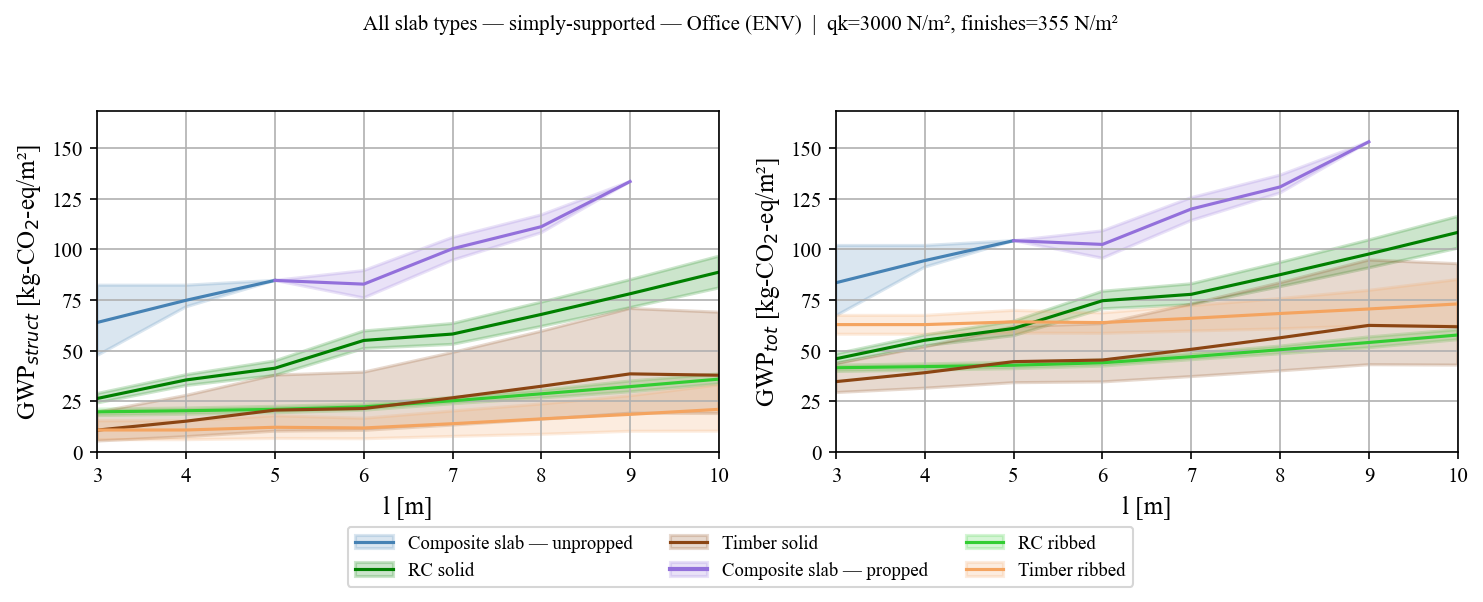
\includegraphics[width=\textwidth]{figures/office/C20/plot_office_1span_ENV_gwpC20.png}
\caption{Office single span, C20/25-only re-run: structural and total GWP versus span for all five floor systems.}
\label{fig:c20_gwp}
\end{figure}
 
\begin{table}[h!]
\centering
\caption{Office single-span composite optimum: baseline (C25/30/C30/37 permitted) versus the C20/25-only re-run.}
\label{tab:c20_sensitivity}
\small
\begin{tabular}{c c c c c c c}
\hline
& \multicolumn{2}{c}{Baseline} & \multicolumn{2}{c}{C20/25 only} & & \\
$L$ [m] & $h$ [mm] & GWP$_{\text{tot}}$ & $h$ [mm] & GWP$_{\text{tot}}$ & $\Delta$GWP & Governing check \\
\hline
3 & 198 & 67.6 & 198 & 67.3 & $-0.3$ & Fire D1 (unchanged) \\
4 & 357 & 91.8 & 357 & 91.3 & $-0.5$ & Fire D4 (unchanged) \\
5 & 279 & 104.7 & 279 & 104.3 & $-0.4$ & Fire D4 (unchanged) \\
6 & 365 & 95.4 & 369 & 95.6 & $+0.2$ & SLS deflection (unchanged) \\
7 & 441 & 114.0 & 447 & 114.3 & $+0.3$ & SLS deflection (unchanged) \\
8 & 504 & 127.4 & 512 & 127.8 & $+0.4$ & SLS deflection (unchanged) \\
9 & 455 & 152.5 & 464 & 153.1 & $+0.6$ & SLS deflection (unchanged) \\
\hline
\end{tabular}
\end{table}
 
The result is that permitting C20/25 changes the single-span composite GWP by less than 0.6\,kg\,CO\textsubscript{2}eq/m\textsuperscript{2} at every span---under 1\,\% of the total---and the governing check is unchanged at every point. More importantly, the sign of the change reverses across the span range, which explains why the intuition that ``the lowest-GWP grade would always be chosen'' does not hold. At the short spans (3--5\,m) the section is governed by the fire thermal-insulation (D1) and minimum-effective-thickness (D4) checks, both of which are independent of concrete grade; the depth is therefore fixed by fire, the same deck and depth are selected, and the only effect of the weaker grade is its lower GWP intensity, giving a marginal \emph{saving} of 0.3--0.5\,kg\,CO\textsubscript{2}eq/m\textsuperscript{2}. From 6\,m upward the section is governed by SLS deflection; here C20/25's lower elastic modulus ($E_{cm}$) reduces the composite stiffness, so the optimiser must add 4--9\,mm of depth to the same deck profile to satisfy the $L/300$ limit, and the additional concrete slightly outweighs the lower per-kilogram intensity, giving a net penalty of 0.2--0.6\,kg\,CO\textsubscript{2}eq/m\textsuperscript{2}. The lowest-GWP grade is therefore selected only where the design is grade-independent; wherever stiffness governs---most of the practical range---a weaker grade is mildly counterproductive.
 
Two conclusions follow. First, the practice-based restriction to C25/30 and C30/37 does not materially affect the reported results: the largest single-span effect of permitting C20/25 is a 0.6\,kg\,CO\textsubscript{2}eq/m\textsuperscript{2} change, negligible against the 1.4--1.8$\times$ gap between the composite slab and the RC flat baseline (Section~\ref{sec:disc_literature}), so none of the comparative rankings or conclusions of Chapter~\ref{fourthchapter} are altered. Second, and perhaps more usefully, the exercise confirms that composite slab GWP is not reduced by specifying a lower-strength concrete: because the design is stiffness-governed over most of the range, any saving from a weaker grade is recovered---or exceeded---by the compensating increase in depth. The restriction is therefore justified not only on practice grounds but also because relaxing it would, if anything, slightly worsen the composite GWP at some spans.

%==============================================================================
\subsection{Swiss market context}
\label{sec:disc_swiss}
%==============================================================================
The deck products in the optimisation database --- Tata Steel ComFlor and Kingspan Multideck --- are manufactured in the United Kingdom and marketed principally in the UK and Irish markets. \cite{RefWorks:2017comflor} describe the ComFlor range as manufactured in the UK and \enquote{readily available} within Europe, while Kingspan Multideck is likewise produced at a single facility in North Yorkshire \citep{RefWorks:kingspan2026multideck}. Neither manufacturer operates a Swiss production or distribution entity.

Profiled steel composite decking is an established product category in Switzerland. Montana Bausysteme AG, a Swiss company of the Tata Steel Europe group since 1964, manufactures and supplies the Holorib\textsuperscript{\textregistered} and SuperHolorib\textsuperscript{\textregistered} composite floor deck ranges from its Swiss facility \citep{Montana_Holorib}. These are re-entrant dovetail profiles designed for composite slab construction per EN~1994-1-1, approved for static and dynamic loading by Swiss building authorities, and have been used in industrial halls, office buildings, multi-storey car parks, and residential construction \citep{Montana_Holorib}. The existence of this Tata Steel-affiliated supply chain suggests that composite steel decking is available in the Swiss market; the specific profiles in the optimisation database (ComFlor~46 to ComFlor~225, Multideck~50 to Multideck~146) are however distinct products from the Montana range and would require independent confirmation of availability before the optimisation results could be applied directly.

ArcelorMittal operates a Swiss-facing market entity that actively markets the Cofraplus\textsuperscript{\textregistered}, Cofrastra\textsuperscript{\textregistered}, and Cofradal\textsuperscript{\textregistered} composite floor deck ranges to Swiss specifiers \citep{AM_schweiz_cofraplus,AM_schweiz_cofradal}. As noted in Section~\ref{sec:epd_deck_assumptions}, ArcelorMittal products were excluded from the main optimisation runs on grounds of EPD inconsistency, not market availability: the single flat-rate area declaration (18.0\,kg\,CO$_2$eq/m$^2$ across all products) is physically implausible and would introduce a systematic bias in favour of the deep-profile configurations where the underestimation is most severe. The availability of ArcelorMittal products in Switzerland therefore reinforces the conclusion that the composite floor slab concept is applicable to Swiss practice, even if the specific GWP results reported here cannot be directly attributed to ArcelorMittal products.

%==============================================================================
\subsection{Further work}
\label{sec:disc_future}
%==============================================================================
Several extensions follow directly from the limitations above.

\paragraph{Cost analysis.} The most significant extension is a cost comparison alongside the GWP comparison. Because the systems differ greatly in construction method---composite construction trades higher material carbon for faster erection and reduced formwork---a cost and programme analysis would test whether the GWP penalty of composite construction is offset by economic and time savings.

\paragraph{Low-carbon steel.}
The composite slab GWP is dominated by the profiled steel deck, which accounts for roughly 40--55\,\% of \gwpstruct{} across the office span range examined (Section~\ref{sec:res_office_breakdown}). Recycled-content or electric-arc-furnace ("green") steel, with a markedly lower GWP intensity than the values used here, would reduce the composite GWP substantially and could narrow the gap to the RC systems.

The baseline EPD intensities used in this study are those of the Tata Steel ComFlor product range (2.79--3.09\,kg\,CO$_2$eq/kg, declared per m$^2$ of profile) and the Kingspan Multideck range (2.50\,kg\,CO$_2$eq/kg, declared per tonne). ArcelorMittal Building Solutions has published an Environmental Product Declaration for deck profiles produced from XCarb\textsuperscript{\textregistered} recycled and renewably produced steel \citep{RefWorks:RefID:121-2025deck}. The declared GWP (A1--A3, total) for a standard deck configuration with a self-weight of 8.89\,kg/m$^2$ is 8.47\,kg\,CO$_2$eq/m$^2$, equivalent to an intensity of 0.95\,kg\,CO$_2$eq/kg --- a reduction of approximately 67\,\% relative to the standard ArcelorMittal deck profile \citep{RefWorks:RefID:115-peters2022epdamc20210146cbb2en} value of $\approx$2.92\,kg\,CO$_2$eq/kg.

To estimate the effect on the optimised office results, the deck EPD intensity in each optimal single-span solution was replaced with the XCarb\textsuperscript{\textregistered} value of 0.95\,kg\,CO$_2$eq/kg while holding all other components (concrete, mesh, trough bars) constant. The results are summarised in Table~\ref{tab:xcarb_sensitivity}. Across the full span range, replacing the conventional deck with a
XCarb\textsuperscript{\textregistered}-equivalent product reduces the structural GWP by 20--42\,\%, with an average reduction of approximately 34\,\%.

\begin{table}[htbp]
  \centering
  \caption{Sensitivity of single-span office to substitution of a low-carbon (XCarb\textsuperscript{\textregistered}-equivalent) deck EPD intensity (0.95\,kg\,CO$_2$eq/kg) for the conventional Tata Steel / Kingspan baseline. All values in kg\,CO$_2$eq/m$^2$.}
  \label{tab:xcarb_sensitivity}
  \small
  \begin{tabular}{ccllrrrc}
    \toprule
    Span & Governing & \multicolumn{2}{c}{GWP$_{struct}$} & \multicolumn{2}{c}{Deck GWP} & \multirow{2}{*}{\shortstack{Reduction\\(kg\,CO$_2$eq/m$^2$)}} & \multirow{2}{*}{\shortstack{Reduction\\(\%)}} \\
    \cmidrule(lr){3-4}\cmidrule(lr){5-6}
    (m) & deck & Baseline & XCarb & Baseline & XCarb \\
    \midrule
    3 & Multideck~60~0.9   & 42.2 & 27.7 & 23.4 &  8.9 & 14.5 & 34.3 \\
    4 & Multideck~80~1.0   & 52.7 & 34.9 & 28.8 & 11.2 & 17.8 & 33.8 \\
    5 & ComFlor~60~0.9     & 64.2 & 44.5 & 29.2 &  9.5 & 19.8 & 30.7 \\
    6 & ComFlor~210        & 75.8 & 44.1 & 46.9 & 15.3 & 31.7 & 41.8 \\
    7 & ComFlor~225        & 94.4 & 61.3 & 49.1 & 16.0 & 33.2 & 35.1 \\
    8 & ComFlor~225        &107.8 & 74.6 & 49.1 & 16.0 & 33.2 & 30.8 \\
    9 & Multideck~146~1.5  &132.9 & 95.3 & 60.8 & 19.8 & 37.7 & 28.3 \\
    \bottomrule
  \end{tabular}
\end{table}

Section~\ref{sec:res_office_breakdown} shows that the optimal single-span RC flat slab (solid) occupies a range of approximately 70--150\,kg\,CO$_2$eq/m$^2$ over the same span range. The XCarb\textsuperscript{\textregistered} values of 28--95\,kg\,CO$_2$eq/m$^2$ indicate that a low-carbon supply chain could bring the composite slab GWP below the RC flat-slab benchmark across virtually the entire span range studied, entirely through a decarbonised steel supply chain and with no structural redesign. This sensitivity highlights the particular responsiveness of the composite system to supply-chain decarbonisation: because the deck dominates the GWP budget, the composite slab is the floor system most immediately affected by --- and most likely to benefit from --- the transition to EAF-route low-carbon steel.

Direct numerical comparison of GWP values across the two standard versions is not formally valid because the impact characterisation factors and system boundaries differ between versions. The XCarb\textsuperscript{\textregistered} EPD covers ArcelorMittal decks, which are not the same products as the Tata Steel ComFlor or Kingspan Multideck profiles optimised in this study; the sensitivity should therefore be read as illustrative of the effect of an EAF-route low-carbon steel supply chain, rather than as a statement that the XCarb\textsuperscript{\textregistered} product specifically achieves the stated structural performance. Subject to these caveats, the calculation represents a credible order-of-magnitude estimate of the carbon savings achievable through supply-chain decarbonisation of the steel deck, and confirms that low-carbon steel is the dominant lever for reducing the embodied carbon of the composite floor system.

\paragraph{End-of-life and module D.} Extending the LCA boundary to include end-of-life recovery (module D) would credit the recyclability and potential demountability of the steel components, and is expected to favour the composite and steel-containing systems relative to the cradle-to-gate comparison used here.

\paragraph{Continuous-span extension of all systems.} Extending the RC ribbed and timber systems to continuous spans would allow a fully consistent cross-system comparison in the continuous configurations, rather than the single-span baselines used at present.

\paragraph{System boundary: slab level only.} The comparison is conducted at the floor-slab level and excludes the supporting structural system. Composite slabs are inherently coupled to a steel frame:  primary and secondary steel beams, which carry substantial embodied carbon, are required and are not present in an equivalent RC flat-slab system. At the full-building scale this represents a material carbon cost not captured in the present comparison, and is expected to widen the GWP gap between composite and RC construction. In the opposing direction, a steel-framed building is substantially lighter than its RC equivalent --- a reduction in superstructure --- which reduces foundation loads and consequently the volume of concrete and reinforcement in the foundations. In ground conditions where piling is substantial, this saving can be material. The net effect at the full-building scale is therefore ambiguous without a complete structural system assessment, and the slab-level comparison presented here should be interpreted accordingly.

\paragraph{Optimiser treatment of propping and shear connection.} Two refinements to the optimisation itself would improve the realism of the comparison. First, the current routine treats propping as a binary fallback, selecting an unpropped section wherever one is feasible and resorting to propping only when no unpropped solution exists, even though propping was shown to yield a lower-GWP section at several spans (Section~\ref{sec:res_office_gov}). Introducing an explicit penalty on propped construction---representing its programme and cost impact---would allow the optimiser to trade the GWP saving of a propped section against its construction-stage disadvantage on a consistent basis, rather than suppressing propped solutions outright. Second, shear connection is presently fixed at the embossment-and-friction shear bond, with end anchorage omitted (Section~\ref{sec:assumptions}). Treating the provision of shear connectors as an additional design variable would let the optimiser thin the deck or reduce its depth where the added connector capacity permits, potentially lowering the overall GWP; the connector GWP would need to be added to the objective so that the trade-off is captured honestly.